\subsection{Branching scheme}

\begin{frame}
  \frametitle{Branching scheme }
  \begin{itemize}
    \vfill
  \item Step 1: ER checker and ER adjustments on current node 
    \begin{itemize}
    \item If checker fails: backtrack
    \item else : go to Step 2
    \end{itemize}
    \vfill    
    \pause
  \item Step 2: Choose $st_i$ or $ft_i$ s.t. $[est_i,lst_i]$ or
    $[eet_i,let_i]$ min
    \vfill
    \pause
  \item Step 3: Create 2 nodes by separating the corresponding
    interval in 2 parts  {\small \it \color{gray!50!black!50} [Carlier
      \& Latapie, 1991]} 
  \end{itemize}
  \begin{overlayarea}{\textwidth}{4cm}
    \only<4>{
      \vfill
      {\it Ex with $st_i$:}
      \begin{center}
        \input{/home/mnattaf/Documents/input_latex/branching.tex}
      \end{center}
    }
    \only<5->{
      \begin{itemize}
      \item Repeat Steps 1--3 until each interval $\inter[est_i][lst_i]$ and $\inter[eet_i][let_i]$ has a size smaller than a given $\epsilon$ (DFS)\\
        \vspace{0.4cm}
        \pause
      \item MILP of the restricted problem
        \begin{itemize}
        \item If MILP solved the problem: STOP
        \item else : backtrack
        \end{itemize}
      \end{itemize}
    }
  \end{overlayarea}
  \vfill
\end{frame}

\subsection{Filtering algorithms}

\begin{frame}
  \frametitle{Energetic reasoning checker}
  {\small adaptation of the energetic reasoning for CuSP
    {\color{gray!50!black!50} \it [Baptiste et al., 2001]}}

  \vspace{0.4cm}
  \pause
  The {\bf slack function} of interval $\inter$ is:
  \begin{gather}
    SL(t_1,t_2)={\color<3>{red!80!black!80}\text{ available space in
      }\inter}-{\color<3>{blue!80!black!80}\text{ total mandatory }} \nonumber\\ 
    {\color<3>{blue!80!black!80}\text{consumption in } \inter}\nonumber
  \end{gather}
  \begin{theorem}
    If there exists an interval on which the slack function is negative then there is no solution
  \end{theorem}
  \vfill
  \onslide<3>{
    \begin{center}
      \begin{tikzpicture}
        [transform shape,xscale=0.7,yscale=0.5]
        [inner sep=0pt]
        \node (O) at (0,0) {};
        \node[right of=O, node distance=6cm] (T) {};
        \node[right of=O, node distance=2cm] (t1) {};
        \node[right of=O, node distance=4cm] (t2) {};
        
        \draw[dashed] (0,4) node[left] {\Large$B$} -- (6,4);

        \draw[->] (O) -- (T);

        \draw[thick,red] (t1) -- (2,4.5);
        \draw[thick,red] (t2) -- (4,4.5);

        \draw[fill=blue!50!black!50] (t1) node[above=2cm,left=0.6cm] {\color{blue!80!black!80} \Large mandatory consumption} rectangle (4.5,4);
        \draw[pattern=north west lines, pattern color=red] (t1) rectangle (4,4) node[below=2cm,right=0.8cm] {\color{red} \Large available resource};
      \end{tikzpicture}
    \end{center}}
\end{frame}

\begin{frame}
  \frametitle{Energetic reasoning checker}
  \vfill
  We define the {\bf mandatory consumption} of $i$ in interval $\inter$ as 
  \[\bb=\min \int_{t_1}^{t_2} b_i(t) dt\]
  \vfill
  In order to compute this quantity we also define the {\bf minimum energy
    consumption} of $i$ in interval $\inter$ as:
  \[\wb=\min \int_{t_1}^{t_2} f_i(b_i(t)) dt\]
\end{frame}


\begin{frame}{Mandatory consumption possible configurations}
  \vfill
\begin{columns}[b]
  \begin{column}{0.45\linewidth}
    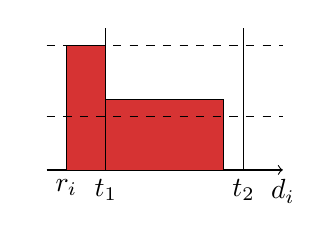
\begin{tikzpicture} [xscale=0.5,yscale=0.45]
      \node (O) at (0,0) {};
      \draw [->] (0,0) -- (6,0);
      \fill[red!80!black!80] (0.5,0) rectangle (1.5,3.5);
      \fill[red!80!black!80] (1.5,0) rectangle (4.5,2);
      \draw (0.5,0) node[below] {$r_i$};
      \draw (6,0) node[below] {$d_i$};
      \draw (1.5,0) node[below] {$t_1$} -- (1.5,4);
      \draw (5,0) node[below] {$t_2$} -- (5,4);
      \draw[dashed] (0,1.5) node[left] {$\bmin$} -- (6,1.5);
      \draw[dashed] (0,3.5) node[left] {$\bmax$} -- (6,3.5);
      \draw (0.5,0) -- (0.5,3.5) -- (1.5,3.5) -- (1.5,2) -- 
      (4.5,2) -- (4.5,0);
    \end{tikzpicture}
    \begin{center}
      {\small left-shifted}
    \end{center}
  \end{column}
\hfill  
\begin{column}{0.45\linewidth}  
  \onslide<2->{
      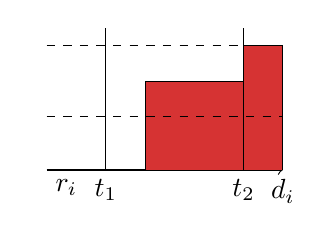
\begin{tikzpicture} [xscale=0.5,yscale=0.45]
        \node (O) at (0,0) {};
        \draw [->] (0,0) -- (6,0);
        \fill[red!80!black!80] (5,0) rectangle (6,3.5);
        \fill[red!80!black!80] (5,0) rectangle (2.5,2.5);
        \draw (0.5,0) node[below] {$r_i$};
        \draw (6,0) node[below] {$d_i$};
        \draw (1.5,0) node[below] {$t_1$} -- (1.5,4);
        \draw (5,0) node[below] {$t_2$} -- (5,4);
        \draw[dashed] (0,1.5) node[left] {$\bmin$} -- (6,1.5);
        \draw[dashed] (0,3.5) node[left] {$\bmax$} -- (6,3.5);
        \draw (6,0) -- (6,3.5) -- (5,3.5) -- (5,2.5) --
        (2.5,2.5) -- (2.5,0);
      \end{tikzpicture}        
      \begin{center}
        {\small right-shifted}
      \end{center}
    }
  \end{column}
\end{columns}
\vfill
\begin{columns}[b]
  \begin{column}{0.45\linewidth}
    \onslide<3->{
      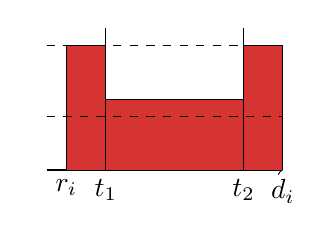
\begin{tikzpicture} [xscale=0.5,yscale=0.45]
        \node (O) at (0,0) {};
        \draw [->] (0,0) -- (6,0);
        \fill[red!80!black!80] (0.5,0) rectangle (1.5,3.5);
        \fill[red!80!black!80] (6,0) rectangle (5,3.5);
        \fill[red!80!black!80] (5,0) rectangle (1.5,2);
        \draw (0.5,0) node[below] {$r_i$};
        \draw (6,0) node[below] {$d_i$};
        \draw (1.5,0) node[below] {$t_1$} -- (1.5,4);
        \draw (5,0) node[below] {$t_2$} -- (5,4);
        \draw[dashed] (0,1.5) node[left] {$\bmin$} -- (6,1.5);
        \draw[dashed] (0,3.5) node[left] {$\bmax$} -- (6,3.5);
        \draw (0.5,0) -- (0.5,3.5) -- (1.5,3.5) -- (1.5,2) --
        (5,2) -- (5,3.5) -- (6,3.5) -- (6,0) ;
      \end{tikzpicture} 
      \begin{center}
      {\small both-shifted 1}
    \end{center}}
  \end{column}
  \hfill
\begin{column}{0.45\linewidth}
    \begin{overlayarea}{0.45\linewidth}{3.5cm}
      \only<4>{
        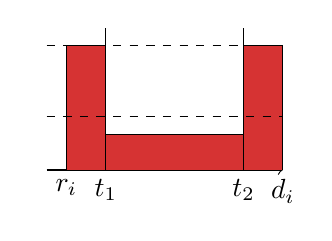
\begin{tikzpicture} [xscale=0.5,yscale=0.45]
          \node (O) at (0,0) {};
          \draw [->] (0,0) -- (6,0);
          \fill[red!80!black!80] (0.5,0) rectangle (1.5,3.5);
          \fill[red!80!black!80] (6,0) rectangle (5,3.5);
          \fill[red!80!black!80] (5,0) rectangle (1.5,1);
          \draw (0.5,0) node[below] {$r_i$};
          \draw (6,0) node[below] {$d_i$};
          \draw (1.5,0) node[below] {$t_1$} -- (1.5,4);
          \draw (5,0) node[below] {$t_2$} -- (5,4);
          \draw[dashed] (0,1.5) node[left] {$\bmin$} -- (6,1.5);
          \draw[dashed] (0,3.5) node[left] {$\bmax$} -- (6,3.5);
          \draw (0.5,0) -- (0.5,3.5) -- (1.5,3.5) -- (1.5,1) --
          (5,1) -- (5,3.5) -- (6,3.5) -- (6,0) ;
        \end{tikzpicture}
      }
      \only<5-> {
        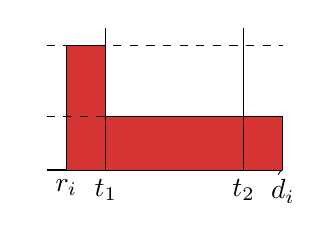
\begin{tikzpicture} [xscale=0.5,yscale=0.45]
          \node (O) at (0,0) {};
          \draw [->] (0,0) -- (6,0);
          \fill[red!80!black!80] (0.5,0) rectangle (1.5,3.5);
          \fill[red!80!black!80] (6,0) rectangle (1.5,1.5);
          \draw (0.5,0) node[below] {$r_i$};
          \draw (6,0) node[below] {$d_i$};
          \draw (1.5,0) node[below] {$t_1$} -- (1.5,4);
          \draw (5,0) node[below] {$t_2$} -- (5,4);
          \draw[dashed] (0,1.5) node[left] {$\bmin$} -- (6,1.5);
          \draw[dashed] (0,3.5) node[left] {$\bmax$} -- (6,3.5);
          \draw (0.5,0) -- (0.5,3.5) -- (1.5,3.5) -- (1.5,1.5) --
          (6,1.5)  -- (6,0) ;
        \end{tikzpicture}
      }
      \onslide<4->{
      \begin{center}
        {\small both-shifted 2}
      \end{center}}
    \end{overlayarea}
  \end{column}
\end{columns}

  \onslide<6>{
    \[\wb = \min ( LS, RS, \max (BS_1,BS_2))\]
  }
\end{frame}

\begin{frame}
  \frametitle{Minimal resource consumption}
  \begin{center}
      \begin{tikzpicture}
  [yscale=0.5,xscale=0.7]
    \node[] (O) at (0,0) {};
    \node[label={[shift={(-0.4,-0.4)}]$b_i^{min}$}] (bmin) at (0,1) {};
    \node[label={[shift={(-0.4,-0.4)}]$b_i^{max}$}] (bmax) at (0,4) {};
    \node[label={[shift={(0,-0.8)}]$t_1$}] (t1) at (4,0) {};
    \node[label={[shift={(0,-0.8)}]$t_2$}] (t2) at (7,0) {};
    \node[label={[shift={(0,-0.8)}]$d_i$}] (di) at (6,0) {};
    \node[label={[shift={(0,-0.8)}]$r_i$}] (ri) at (1,0) {};
    
    \draw[->] (O.center) -- (8,0);
    \draw (O.south) -- (bmax.north);
    \draw (bmin.center) -- (8,1);
    \draw (bmax.center) -- (8,4);
    \draw[fill=white] (ri.center) rectangle (4,4);
    \draw[pattern=north west lines] (ri.center) rectangle (4,4);
    \draw[fill=white] (t1.center) rectangle (5,1.5);
    \draw[pattern=north west lines] (t1.center) rectangle (5,1.5);
    \draw(di.south) -- (di.center);
    \draw(ri.south) -- (ri.center);
    \draw[thick,color=green!80!black!80] (t1.south) -- (4,4.1);
    \draw[thick,color=green!80!black!80] (di.south) -- (6,4.1);
    \draw[] (t2.south) -- (7,4.1);

    \draw[color=green!80!black!80,thick,decorate,decoration={brace,raise=0.1cm}] (4,4) -- (6,4) node[above=0.2cm,pos=0.5] {J};

  \end{tikzpicture}

  \end{center}
  \vfill
  \pause
  \textbf{Question : }
  How can we bring an {\bf energy} $\mathbf{\wb}$ to $i$ in interval $J$ by consuming
  {\bf as few resource} as possible? 
  \vfill
  \pause
  \begin{align*}
    \text{ min }& \int_{J} b_i(t)dt  &\\
    \text{ s.t. } & \int_{J}f_i(b_i(t))dt \ge  \underline{w}(i,t_1,t_2)& \\
                &  \bmax \ge b_i(t) \ge \bmin \qquad \forall t \in J
  \end{align*}
  \vfill
\end{frame}

\begin{frame}
  \frametitle{Analytic expression of $\bb$}
  \vfill
  \begin{itemize}
  \item  \textbf{Question : }
    How can we bring an energy $\wb$ to $i$ in interval $J$ by consuming as few resource as possible?
    \vfill
    \begin{align*}
      \text{ min }& \int_{J} b_i(t)dt  \\
      \text{ s.t. } & \int_{J}f_i(b_i(t))dt \ge  \underline{w}(i,t_1,t_2) \\
                  &  \bmax \ge b_i(t) \ge \bmin\qquad \forall t \in J
    \end{align*}
    \vfill
  \item Theorem "piecewise constant $b_i(t)$" $\Rightarrow$ there is a constant $b_{i} > 0 $
    s.t. 
    \pause
    \begin{align*}
      \text{min }  & \int_{J} b_i\,dt  \\
      \text{s.t } & \int_{J}f_i(b_i)\,dt \ge
                    \underline{w}(i,t_1,t_2)\\
                   & \bmax \ge b_i \ge \bmin
    \end{align*}
  \end{itemize}
  \vfill
\end{frame}

\begin{frame}
  \frametitle{Analytic expression of $\bb$}
  \vfill
  $\bullet$ if $f_i$ is linear, i.e. of the form $f_i(b)= a_i*b+c_i$ :
  \pause
  \begin{align*}
    \text{min }  & \int_{J} b_i\,dt  \\
    \text{s.t } & \int_{J}(a_i*b_i+c_i)\,dt \ge
                  \underline{w}(i,t_1,t_2)\\
                 & \bmax \ge b_i \ge \bmin
  \end{align*}
  \pause
  { \color{blue!80!black!80}
    $\boldmath{\Rightarrow  \underline{b}(i,t_1,t_2)= \max ( |J|\bmin, \frac{1}{a_i}( \underline{w}(i,t_1,t_2)-|J|c_i))}$}.
  
\end{frame}

\begin{frame}
  \frametitle{Analytic expression of $\bb$}
  \vfill
  $\bullet$  if $f_i$ is concave and piecewise linear, i.e. of the form
  $f_i(b)=a_{ip}*b+c_{ip}, \forall p \in {\cal P}$:
  \pause

  \begin{align*}
    \text{min }  & \int_{J} b_i\,dt  \\
    \text{s.t } & \int_{J}(a_{ip}*b_i+c_{ip})\,dt \ge
                  \underline{w}(i,t_1,t_2) \qquad \forall p \in
                  {\cal P}\\
                 & \bmax \ge b_i \ge \bmin
  \end{align*}
  \pause
  { \color{blue!80!black!80}
    $\boldmath{\Rightarrow  \underline{b}(i,t_1,t_2)= \max ( |J|\bmin, \max_{p
        \in {\cal P}} \frac{1}{a_{ip}}( \underline{w}(i,t_1,t_2)-|J|c_{ip}))}$}
  \vfill
  \begin{prop}
    The slack function of $[t_1,t_2]$ can be computed in linear time
    for the CECSP$_{lin}$ and $O(\#tasks.|{\cal P}|)$ for the CECSP$_{cpwl}$.
  \end{prop}
\end{frame}


\begin{frame}
  \frametitle{Relevant intervals}
  {\bf Question: } For which intervals $\inter$ we have to compute $SL(t_1,t_2)$?\\
  \vfill
  \pause
  $\rightarrow$ Analysis of the variation of the slack function (
  {\small CuSP : \it \color{gray!50!black!50} [Derrien \& Petit, 2015]})\\
  \vfill
  \begin{block}{Slack function}
    \centering $SL(t_1,t_2)=B(t_2-t_1) - \sum_{i \in A} \bb$
  \end{block}
  \vspace{0.8cm}
  $\rightarrow$ Variation of $SL(t_1,t_2)$ depends on variation of 
  $\sum_{i \in A} \bb$
  \vfill 
  $\rightarrow$ Polynomial number of intervals (checker + filter)  \vfill 
\end{frame}

% \begin{frame}{Example}

%   {\small
%   Case: $W_i \ge f_i(\bmax)( let_i-est_i)$ and $est_i < t_1 \le \frac{est_if_i(\bmax)-let_i f_i(\bmin)+W_i}{f_i(\bmax)-f_i(\bmin)}$}
%   \begin{center}
%     \begin{tikzpicture}
%       [yscale=0.2,xscale=0.4]
%       \node (O) at (0,0) {};
%       \draw[->] (-1,0) -- (18,0) node[below] {$t_2$};
%       \draw[->] (-1,0) -- (-1,15) node[left] {$\bb$};

%       \draw (0,1) -- (3,1) -- (6,6) -- (10,8) -- (13,13) -- (17,13);

%       \draw[dashed] (3,0) node[below] {$ lst_i$} -- (3,1);      
%       \draw[dashed] (6,0) node[below] {$\Delta(t_1)$} -- (6,6);  
%       \draw[dashed] (10,0)  -- (10,8);  
%       \draw[dashed] (13,0) node[below] {$ let_i$} -- (13,13);
%     \end{tikzpicture}
%   \end{center}
%   {\small with $\Delta(t_1)=\frac{W_i-f_i(\bmin)let_i
%   +t_1f_i(\bmax)}{f_i(\bmax)-f_i(\bmin)}$}

%   \vspace{0.2cm}

%   $\rightarrow$ We have to consider $[t_1,\Delta(t_1)]$ and $[t_1,d_i]$


%   \vspace{0.2cm}
%   $\rightarrow$ Polynomial number of interval (checker and filter)
%   \vfill 
% \end{frame}

\subsubsection{Energetic reasoning filter}

\begin{frame}
  \frametitle{Time window adjustments}
  \vspace{0.4cm}
  \begin{center}
    \begin{tikzpicture}
 [yscale=0.5,xscale=0.9]
 \node[] (O) at (0,0) {};
 \node[label={[shift={(-0.4,-0.4)}]\small $b_i^{min}$}] (bmin) at (0,1) {};
 \node[label={[shift={(-0.4,-0.4)}]\small $b_i^{max}$}] (bmax) at (0,4) {};
 \node[label={[shift={(-0.4,-0.4)}]\small $B$}] (B) at (0,6) {};
 \node[label={[shift={(0,-0.8)}]\small $t_1$}] (t1) at (2.5,0) {}; 
 \node[label={[shift={(0,-0.8)}]\small $est_i$}] (ri) at (1.5,0) {};
 \node[label={[shift={(0,-0.8)}]\small $t_2$}] (t2) at (6,0) {};
 %\node[label={[shift={(0,-0.8)}]\small $d_i$}] (di) at (7,0) {};
 

\onslide<5->{
\draw[pattern=north west lines, pattern color=red!80!black!80] (4.25,1) --(6,1) -- (6,6) -- (2.5,6) -- (2.5,0) -- (4.25,0) -- cycle;;
%\draw[color=white,pattern=north west lines, pattern color=red!80!black!80] (4.25,0) rectangle (2.5,6);
\draw[pattern=north east lines, pattern color=blue!80!black!80] (4.25,0) rectangle (6,1);
\draw[pattern=north east lines, pattern color=black!80] (6,0) rectangle (7.5,4);
\draw[white,dashed] (6,0) rectangle (7.5,4);
} 
  \draw[->] (O.center) -- (8,0);
  \draw (O.south) -- (B.north);
  \draw (B.center) -- (8,6);
  \draw[dashed] (bmin.center) -- (8,1);
  \draw[dashed] (bmax.center) -- (8,4);
  \draw(ri.south) -- (ri.center);
%  \draw(di.south) -- (di.center);
  \draw[thick] (t1.south) -- (2.5,6.1);
  \draw[thick] (t2.south) -- (6,6.1);
  \onslide<1>{
    \draw[pattern=north west lines, pattern color=red!80!black!80] (t1.center) rectangle (6,6);}
  \onslide<2-4>{
    \draw[pattern=north west lines, pattern color=red!80!black!80] (2.5,0.5) rectangle (6,6);}
  \onslide<3-4>{
\draw[pattern=north east lines, pattern color=blue!80!black!80] (1.5,0) rectangle (2.5,4);}
  \onslide<3>{
\draw[pattern=north east lines, pattern color=blue!80!black!80] (2.5,0) rectangle (6,2);
}
\onslide<4>{
\draw[pattern=north east lines, pattern color=blue!80!black!80] (6,0) rectangle (7,4);
\draw[pattern=north east lines, pattern color=blue!80!black!80] (2.5,0) rectangle (6,1);
} 

\end{tikzpicture}

  \end{center}
  \vfill
  \begin{block}{Adjustments}
    if {\color<2-3>{red!80!black!80} available space for $i$}$<${\color<3-4>{blue!80!black!80} consumption of $i$ starting at $est_i$}  then
    \[\textcolor<5>{red!80!black!80}{est_i \text{ can be adjusted}}\]
  \end{block}
  \vfill
\end{frame}

\subsubsection{Other filtering algorithms}

\begin{frame}{Other filtering algorithms}
  \vfill
  \begin{itemize}
  \item {\bf \color{blue!80!black!80} Simple reasoning: } adaptation of
    {\bf time-table} reasoning and {\bf disjunctive} reasoning
    \vfill
    {\color{gray!80!black!80}{\it Idea: } Consider rectangular task with two modes

      $\rightarrow (\bmax, W_i/f_i(\bmax))$ maximal consumption/minimal time

      $\rightarrow (\bmin, W_i/f_i(\bmin))$ minimal consumption/maximal
      time}
    \vfill
    \pause
  \item {\bf \color{blue!80!black!80} Combined/Extended reasoning: }
    adaptation of the {\bf time-table disjunctive} reasoning (TTDR) and
    new {\bf time-table flow-based} satisfiability test (TTFB)
    \vfill
    {\color{gray!80!black!80}{\it Idea: } TTDR $\rightarrow$ same as TT and DR
      
      TTFB $\rightarrow$ Flow-based LP with minimal consumption $\bmin$ in
      ${[}lst_i ,eet_i{]}$ and $0$ outside}
  \end{itemize}
\end{frame}


\subsection{Computational results}

\begin{frame}
  \frametitle{Branching scheme }
  \begin{itemize}
    \vfill
  \item Step 1: ER checker and ER adjustments on current node 
    \vfill    
  \item Step 2: Choose $st_i$ or $ft_i$ s.t. $[est_i,lst_i]$ or
    $[eet_i,let_i]$ min
    \vfill
  \item Step 3: Create 2 nodes by separating the corresponding
    interval in 2 parts {\small \it \color{gray!50!black!50} [Carlier \& Latapie, 1991]}
    \vfill
  \item{\color{red!80!black!80} Repeat Steps 1--4 until each interval $\inter[est_i][lst_i]$ and $\inter[eet_i][let_i]$ has a size smaller than a given $\epsilon$ (DFS)}
    \vfill
  \item MILP of the restricted problem
    \begin{itemize}
    \item If MILP solved the problem: STOP
    \item else : backtrack
    \end{itemize}
  \end{itemize}
  \vfill
\end{frame}


\begin{frame}
  \frametitle{Computational results}
  \vfill
  \begin{block}{Instance generation}
    \begin{itemize}
    \item 20 instances of 20, 25, 30 tasks. 
    \item Family 1: random  $a_i$ and $c_i,\ \forall i \in A$, in ${[}1,10{]}$
      and $W_i$ in ${[}0,f_i(W_i){]}$

      Family 4: $f_i(b_i(t))= b_i(t)$
    \item $\epsilon = 2.5$ 
    \end{itemize}
  \end{block}
  \vfill
  \pause
  \begin{block}{Configuration}
    \begin{itemize}
    \item Intel Core i7-4770 processor with 4 cores and 8Go of RAM
    \item OS: 64-bit Ubuntu 12.04
    \item MILP resolution: CPLEX 12.6  
    \item BB : C++ and CPLEX at each leaf
    \item time limit: 7200 seconds
    \end{itemize}
  \end{block}
  \vfill
\end{frame}

\begin{frame}
  \frametitle{Computational results} 
  \begin{center}

    \begin{tabular}{|c|cc|cc|}
      \hline
      \#tasks & \multicolumn{2}{c|}{On/Off Model}&
                                                    \multicolumn{2}{c|}{Hybrid
                                                   BB}\\ 
      \hline 
              & time(s) &\%solv. & time & \%solv.\\ 
      \hline
      \multicolumn{5}{|c|}{Family 1}\\
      \hline 
      $20 $&  \alt<2>{$11.56$}{$\mathbf{11.56}$} & \alt<1>{$100$}{$\mathbf{100}$} &$660.21$  &$90$\\ 
      $25 $& \alt<2>{$58.79$}{$\mathbf{58.79}$} &
                                                  \alt<1>{$100$}{$\mathbf{100}$} & $821.9$ & $88$ \\ 
      $30 $& $1582.9$ & $80$ & \alt<2>{$112.58$}{$\mathbf{112.58}$} &
                                                                      \alt<1>{$ 100$ }{$\mathbf{100}$}\\  
      \hline 
      \multicolumn{5}{|c|}{Family 4}\\
      \hline 
      $20 $& \alt<2>{$734.04$}{$\mathbf{734.04}$} & \alt<1>{$90.9$}{$\mathbf{90.9}$}
              & $1617.07$ & $77$\\  
      $25 $& $2102.85$ & $77.8$ & \alt<2>{$104.9$ }{$\mathbf{104.9}$}&\alt<1>{$100 $ }{$\mathbf{100}$}\\ 
      $30 $& $4483.4$&$60$ & \alt<2>{$1749.76$}{$\mathbf{1749.76}$} &\alt<1>{$77$ }{$\mathbf{77}$}\\  
      \hline 
    \end{tabular}
  \end{center}
\end{frame}




